\chapter{Log in to \ares}
\label{ch:login}
There are two ways to access \ares system. While we suggest using the most straightforward approach, you are free to option for the another way, especailly if you are an experience NYU Classes user. 
\section{Fly to it}
\label{sec:diret way}
The most straightforward way to log in to \ares is using your NYU credentials to visit \url{https://ares.library.nyu.edu}. Similarly, you can also access \ares through the \button{\crtab} tab on the library's homepage, which links to the same place.

\vspace*{3ex}
\begin{figure}[h]
    \centering
    
\includegraphics[width=\linewidth]{tab2}
    \caption{\footnotesize The Course Reserve Tab}
    \label{fig:Course Reserve Tab}
\end{figure}
\vspace*{2ex}


\section{By an old friend}
\label{sec:nyu classes}
Another way to log in is through NYU Classes. Course reserves link can be added to any NYU Classes course so that the Course Reserves link appears within the NYU Classes course. The following steps show how (\autoref{fig:Course Reserves Option}):
% \tcbdocmarginnote{\href{https://youtu.be/wUEl8KrMz14}{video tutorial}}
\begin{enumerate}
    \item Click on {\imp Settings} on the left navigation bar; 
    \item Select {\imp Add/Edit Tools} on the top menu; 
    \item Check the box \checkbox{\checkmark} next to {\imp Course Reserves}
    \item Scroll down and click \nyuclass{Continue} at the bottom; then click \nyuclass{Finish} on the confirmation web page.
\end{enumerate}

\begin{figure}[t]
    % \centering
    \begin{subfigure}{\textwidth}
        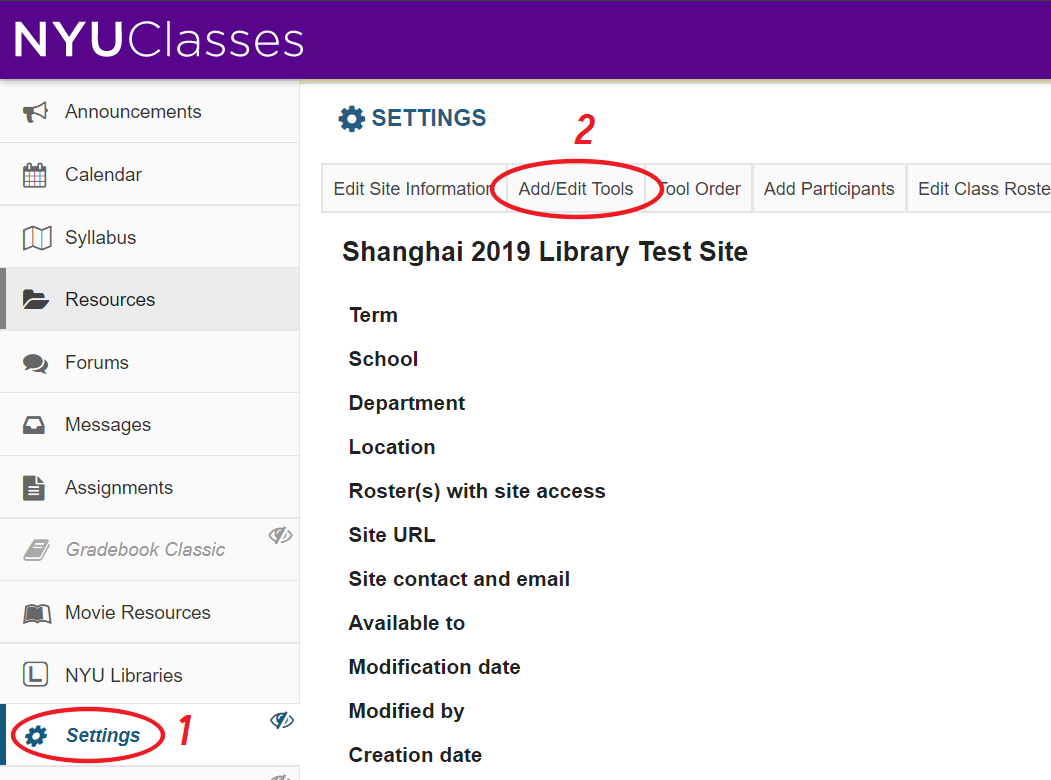
\includegraphics[width=\linewidth]{nyuclass1}
        \caption{Add Reserve Option}
        % \hspace*{1.5cm}
        \label{fig:Add Reserve Option}
    \end{subfigure}
    
    \begin{subfigure}{\textwidth}
        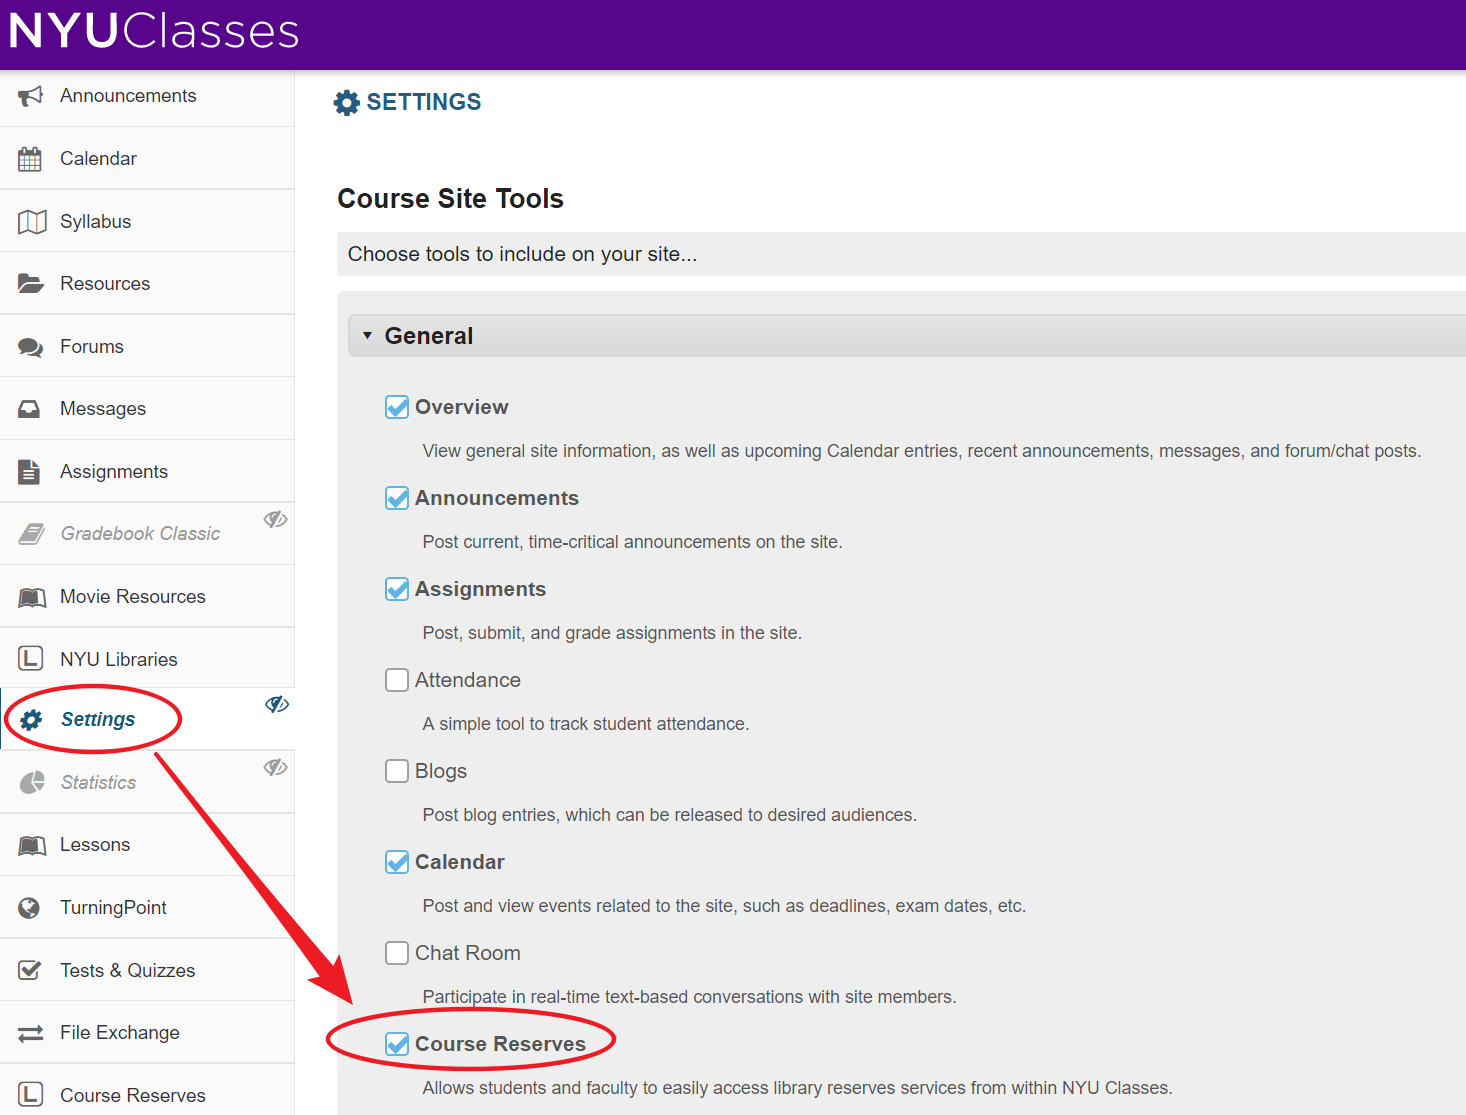
\includegraphics[width=\linewidth]{nyuclass2}
        \caption{Enable Reserve Option}
        \label{fig:Enable Reserve Option}
        \end{subfigure}
\caption{Enabling Course Reserves in NYU Classes}
\label{fig:Course Reserves Option}
\end{figure}

You are all set! Clicking on the Course Reserve link, instructors can add reserve items to the course while student users can view the available items for the course without any additional login to Ares.